\documentclass[aspectratio=1610, 13pt]{beamer}
\usepackage{verbatim}
\usepackage{amsmath}
\usepackage{amsthm}
\usepackage{multicol}
\usepackage{graphics}
\usepackage{color}
\usepackage{stmaryrd}\usefonttheme[onlymath]{serif}

\usepackage{listings}
\usepackage{color}
\renewcommand\lstlistingname{Quelltext} % Change language of section name
\lstset{ % General setup for the package
    language=Perl,
    basicstyle=\small\sffamily,
    numbers=left,
     numberstyle=\tiny,
    frame=tb,
    tabsize=4,
    columns=fixed,
    showstringspaces=false,
    showtabs=false,
    keepspaces,
    commentstyle=\color{red},
    keywordstyle=\color{blue}
}


\title{Progess Report}
\date{\today}
\author{Presentor: Xie Li}
\begin{document}
\maketitle

\begin{frame}\frametitle{Overview}
\begin{itemize}
\item A simple example for symbolic execution.
\item Modifying SMACK: symbolic execution for \texttt{malloc} and \texttt{bitcast} from pointer to pointer(with assumption).
\item Proposed a framework based on problems encountered.
\end{itemize}
\end{frame}

\begin{frame}[fragile]{The Simplest Example}
    Here is the simplest example in C related to memory operations.
\begin{lstlisting}
int main(){
    int *i;
    i = (int*)malloc(sizeof(int));
    free(i);
}

\end{lstlisting}
And its corresponding LLVM IR:
\begin{lstlisting}
define dso_local i32 @main() {
    %1 = call noalias i8* @malloc(i64 4)
    %2 = bitcast i8* %1 to i32* 
    %3 = bitcast i32* %2 to i8*
    call void @free(i8* %3)
    ret i32 0
}

\end{lstlisting}

\end{frame}


\begin{frame}{Symbolic Execution Rules}
    
Symbolic Heap: $Q\equiv \Pi\mid \Sigma$
\begin{align*}
&\Pi\mid \Sigma\Rightarrow_{\{x:=\mathtt{malloc}(e)\}} \Pi[x'/x]\mid \Sigma[x'/x] * x\mapsto e[x'/x] * \mathtt{blk}(x+1,x+1+e[x'/x])\\
&\Pi\mid \Sigma_0 *x\mapsto e*\mathtt{blk}(x+1,x+1+e)*\Sigma_2\Rightarrow_{\{\texttt{free}(x)\}} \Pi \mid \Sigma_0 *\Sigma_2\\
\end{align*}
\begin{center}
    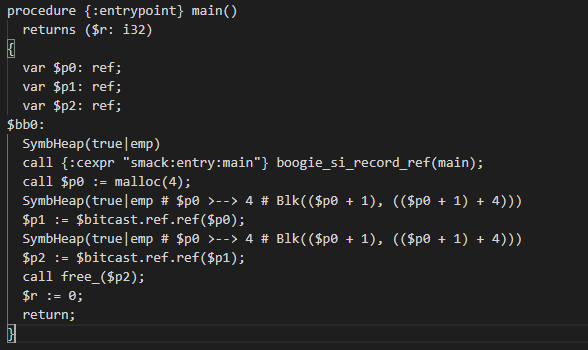
\includegraphics[scale=.65]{boogie.PNG}
\end{center}


\end{frame}

\begin{frame}{Framework}
\begin{center}
    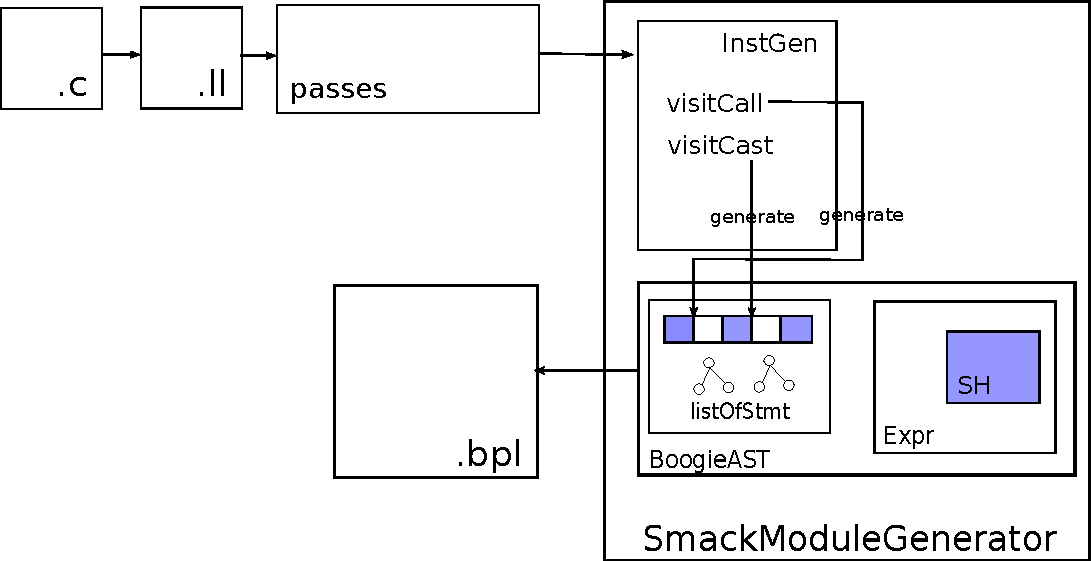
\includegraphics[scale=.7]{smack.pdf}
\end{center}
\end{frame}

\begin{frame}{Framework}
    
\begin{center}
    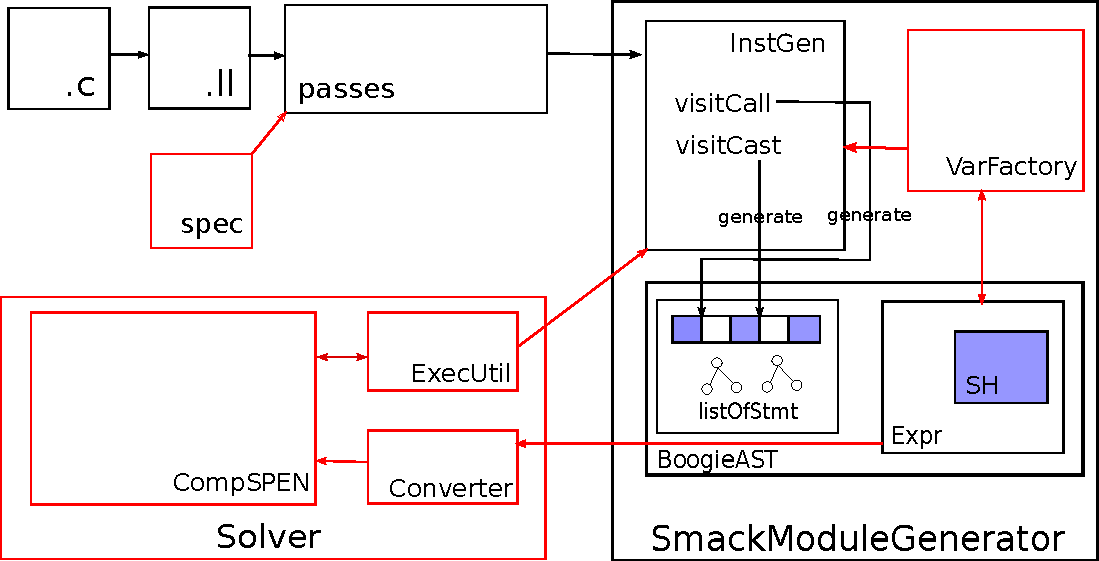
\includegraphics[scale=.7]{gen.pdf}
\end{center}
\end{frame}

\begin{frame}{TODOs}
\begin{itemize}
    \item Translation: Incrementally investigate the instruction for execution. Thoroughly went through \texttt{InstGen} and find data structure available for the symbolic execution.
    \item AST: Implement a \texttt{VarFactory} module for better syntactical variable manipulation, extend \texttt{BoogieAST} to get more information and unify the basic memory unit.
    \item VCGen: Add \texttt{Solver} component to assist symbolic execution and together with \texttt{spec} for verification condition generation.
\end{itemize}
\end{frame}

\begin{frame}{Current Problems and Needs}
\begin{itemize}
    \item Symbolic Execution: Directly using \textsc{Z3}/\textsc{CompSPEN} or use \texttt{BoogieAST}? Concentrate more on syntax or semantic? The problem of \texttt{free}.
    \item The conversion between different types of basic data structure: intermediate language unifying the basic unit of memory.
    \item Feasibility of current framework.
\end{itemize}
\end{frame}



\end{document}